\documentclass[a4paper,11pt, twocolumn]{article}
\usepackage{amsmath}
\usepackage{graphicx}


\begin{document}

\title{Linear Regression on Boston Housing Data}
\author{Alun Meredith}
\maketitle

\begin{abstract}
In this lab we explore radial basis functions as a method for non-linear regression analysis and compare its performance to linear regression methods from lab four for two different datasets.
\end{abstract}

\section{Method}
In both linear regression and Radial Basis Functions (RBF) we construct a model of the data and train that model to best represent the data by minimising some error function representing the distance between the observations of a training set and the model. The distinction between the two methods is that linear regression has a model of an m dimensional straight line whereas LBF has a collection of points (centres) as its model and therefore the cost function is a measure of the weighted distance between those centres and the observations (eq.\ref{eq:model}).

\begin{align}
	\label{eq:model}	
	g(\mathbf{x}) &= \sum_{k=1}^K\lambda_k\phi(||\mathbf{x-c_k}||)\\
	\label{eq:pdf}
	\phi(c_k,x) &= e^{{-\frac{(x-c_k)^2}{2\sigma^2}}}\\
	\label{eq:weights}
	\lambda &= D / y
\end{align} 

To construct a regression using RBF we first normalise the data, subtracting the mean and dividing by the standard deviation for each variable. The purpose of normalising the data is the make sure that variables with large values don't dominate variables with small values. This is weighted against the idea that some variables with small values are more likely to have genuinely small effects however the model can often between these so it is valuable to normalise the data. 

To construct the position of the centres a K-means clustering algorithm was used. We initialise K cluster centres randomly and assign each observation to its nearest cluster before recomputing the position of the clusters as the mean position of the points associated with that cluster. This is repeated until the clusters no longer move. 

Just like in linear regression a method for evaluating the cost must be chosen. These methods are the Radial Basis Functions and many different functions can be chosen here to model the data in different ways. In this case we chose a Gaussian model as it enabled us to use the K-means clustering to compute the centres and confers a sense of locality. In this case we must choose the value for $\sigma$ to parametrise these functions. We will consider a simple approximation of the variance in the data by taking a sample of 10 pairs of observations and computing the average euclidean distance between the two. 

Using these RBFs we can compute the probability density of each of the K centres on each of the n observations (eq.\ref{eq:pdf}). This is our measure of distance from the model and gives us a Design Matrix. 

Finally we train the weights ($\lambda$) of each Radial basis function as the effect its PDF has on the target value $y$ (eq.\ref{eq:weights}).
\section{Parameters}
When we build a Gaussian RBF there are two parameters to consider, the number of clusters (K) and the width of the Gaussian $\sigma$. It is not immediately obvious what values of these parameters we should choose to produce a model which best represents the data, so we vary these parameters and see how they effect the error. 

\begin{figure}[ht]
	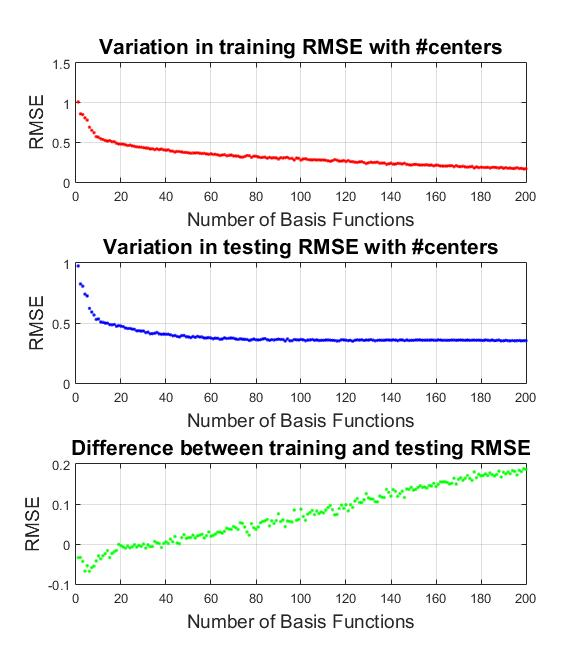
\includegraphics[width=\linewidth]{VaryingK.jpg}
	\centering
	\caption{Variation in testing and training RMSE error with number of RBF clusters K}
		\label{fig:VaryingK}
\end{figure}

As the figure (\ref{fig:VaryingK}) shows increasing the number of centres continuously improves the accuracy on the training set but after a point has no more effect on the accuracy on the testing set. Large difference between training and testing set like this is indicative of high variance (overfitting) occurring in our model. This makes logical sense as when the centres per observation approaches 1 you will have a centre under each observation. Equally when there are few numbers of centres we have high bias in that our model is overly restricted and cannot perform well on either dataset. To balance these two effects we will choose the smallest number of centres which where the testing set RMSE no longer improves substantially in this case around 50. 

\begin{figure}[ht]
	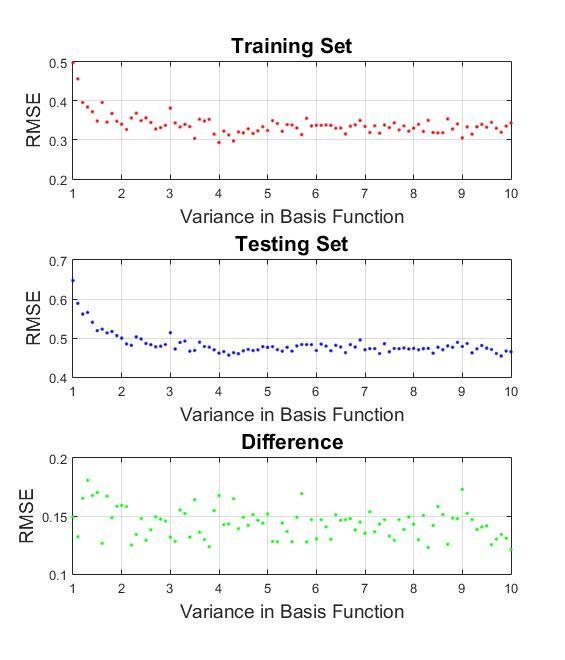
\includegraphics[width=0.8\linewidth]{VaryingSigma.jpg}
	\centering
	\caption{Variation in testing and training RMSE error with variance of Basis Functions $\sigma$}
		\label{fig:VaryingK}
\end{figure}

For varying the value of sigma we see that similarly having low values performs poorly on both the training set and testing set, however neither the training set or test set seem to have visible improvements after the range of about 4. Considering the average value of Sigma approximated through the euclidean distance between two points method was 4.70 (average of 1000 samples) it seems appropriate to continue using this method as long as we are taking an average of a small sample to mitigate some of the random effects. 


\end{document}